\chapter{Introduction}
\label{chap:introduction}
%\ac{PaaS}

Cloud computing has changed in the last years the computing resources consumption and delivery model in the IT industry, leading to offer them as services which can be can be accessed over the network. The idea of virtualizing resources and provide them on demand to the users, like water, electricity, etc. under a metered service aims to deliver computing as a utility. Users are offered a single system view in a fully virtualized environment where computing resources seem unlimited, and can be accessed through Web interfaces and standardized protocols. Cloud providers target to maximize their benefits by maximizing the resources usage with a minimum management effort or human interaction, while the Cloud consumers can significantly reduce their capital expenditures in their IT infrastructure by outsourcing the demanded computational and storage resources to a Cloud environment.

In the following sections we discuss the problem statement and motivating scenario this thesis relies on. 

\section{Problem Statement}
\label{sec:problemstatement}     

A multi-tenant aware architecture in a Cloud environment is one of the main keys for profiting in a Cloud infrastructure. Virtualization and simultaneously usage of resources by multiple users allow Cloud providers to maximize their resources utilization. However, a multi-tenant environment requires isolation between the different users at different levels: computation, storage, and communication \cite{EnablingMT}. Furthermore, the communication to and from the Cloud infrastructure must support different protocols. 

Migration of an application to the Cloud can be divided into four different migration types: component replacement with Cloud offerings, partial migration of functionalities, migration of the whole software stack of the application, and cloudifying the application \cite{andrikopoulos2013}. In this diploma thesis we focus on the needed support when the first migration type takes place. For example, due to an explosive data growth a tenant may decide at some point in time to migrate and host his local business data in a Cloud storage infrastructure, while maintaining his application's business logic on-premise. Bachmann provides a prototype which assists the tenant during the data migration process from a local storage system to a Cloud data store, and between Cloud data stores \cite{bachmann2012}. However, as described before his work covers the migration process, but it does not provide data access or data modification after the migration. 

An Enterprise Service Bus is a central piece in a \ac{PaaS} environment for providing flexible and loosely coupled integration of services as well as multi-tenant aware and multi-protocol communication between services. In this diploma thesis we extend the multi-tenant aware prototype of an \ac{ESB} produced in \cite{Muhler2012}, \cite{Essl2011}, and \cite{gomez2012}. The final prototype must provide multi-tenant and multi-protocol communication support, and transparent Cloud data access to tenants who migrate their application data partially or completely to the Cloud. 

The use of an intermediate component in data transfer may have a negative impact on the overall data processing in an application. For this reason, we provide an evaluation using example data from an existing TPC benchmark in order to investigate the impact on the performance and to propose future optimizations \cite{tcpbenchmark}.
\section{Motivating Scenario}
\label{sec:motivatingscenario}

IT industries aim to reduce their budget in expensive hardware investment and maintenance, e.g. Database Management Systems, while maintaining data access and persistency over time. In order to fulfill a budget reduction while maintaining their data and database system requirements, the data can be migrated to different Cloud storage providers available nowadays in the market. Considering the application's migrations types discussed in \cite{andrikopoulos2013}, migrating local data to the Cloud, and then accessing it from the application's hosted on-premise, can be considered as a \term{partial or complete replacement of components with Cloud offerings}. Such migration requires a reconfiguration, rewiring, and adaptation activities on both the migrated and non-migrated components.

The \term{Cloud Data Migration Application} assists the user in the migrating decision and process of local data to a Cloud storage provider, or from two different Cloud storage providers \cite{bachmann2012}. It contains a registry of the different available Cloud data stores, e.g. Amazon Dynamo DB  \cite{amazondynamodb}, Amazon RDS \cite{amazonrds}, Google Cloud SQL \cite{googlecloudsql}, and detects possible incompatibilities between the source and target data sources prior to the migration process.

Migration of data can be either seen as the migration of only the Data Layer, or as a part of the migration of the whole application \cite{andrikopoulos2013}. The approach we consider as the start point in this diploma thesis is the migration of the Data Layer, which contains two sublayers: the \term{Database Layer (DBL)} and the \term{Data Access Layer (DAL)}. The DBL contains the database information, e.g. location, access credentials, etc., and gives the DAL a direct communication support to the database server. The DAL provides simplified access support to the upper layers of the data stored in a backend database. However, migrating the Data Layer to the Cloud implies adaptations and rewiring of the original application. One of our main goals in this diploma thesis is to minimize the needed adaptations in the non-migrated and migrated components by providing a transparent access to the user's data migrated to a Cloud datastore. 

As the Enterprise Service Bus is an established integration middleware for services in Service-Oriented Architectures (SOA), and due to its multi-protocol support and reliable internal messaging routing, we use it as a central piece for providing a multi-tenant aware, transparent and reliable communication support between the on-premise and the off-premise layers of the application.

%\cite{4CaaSt} \ac{HTTP}

\begin{figure}[htb]
	\centering
		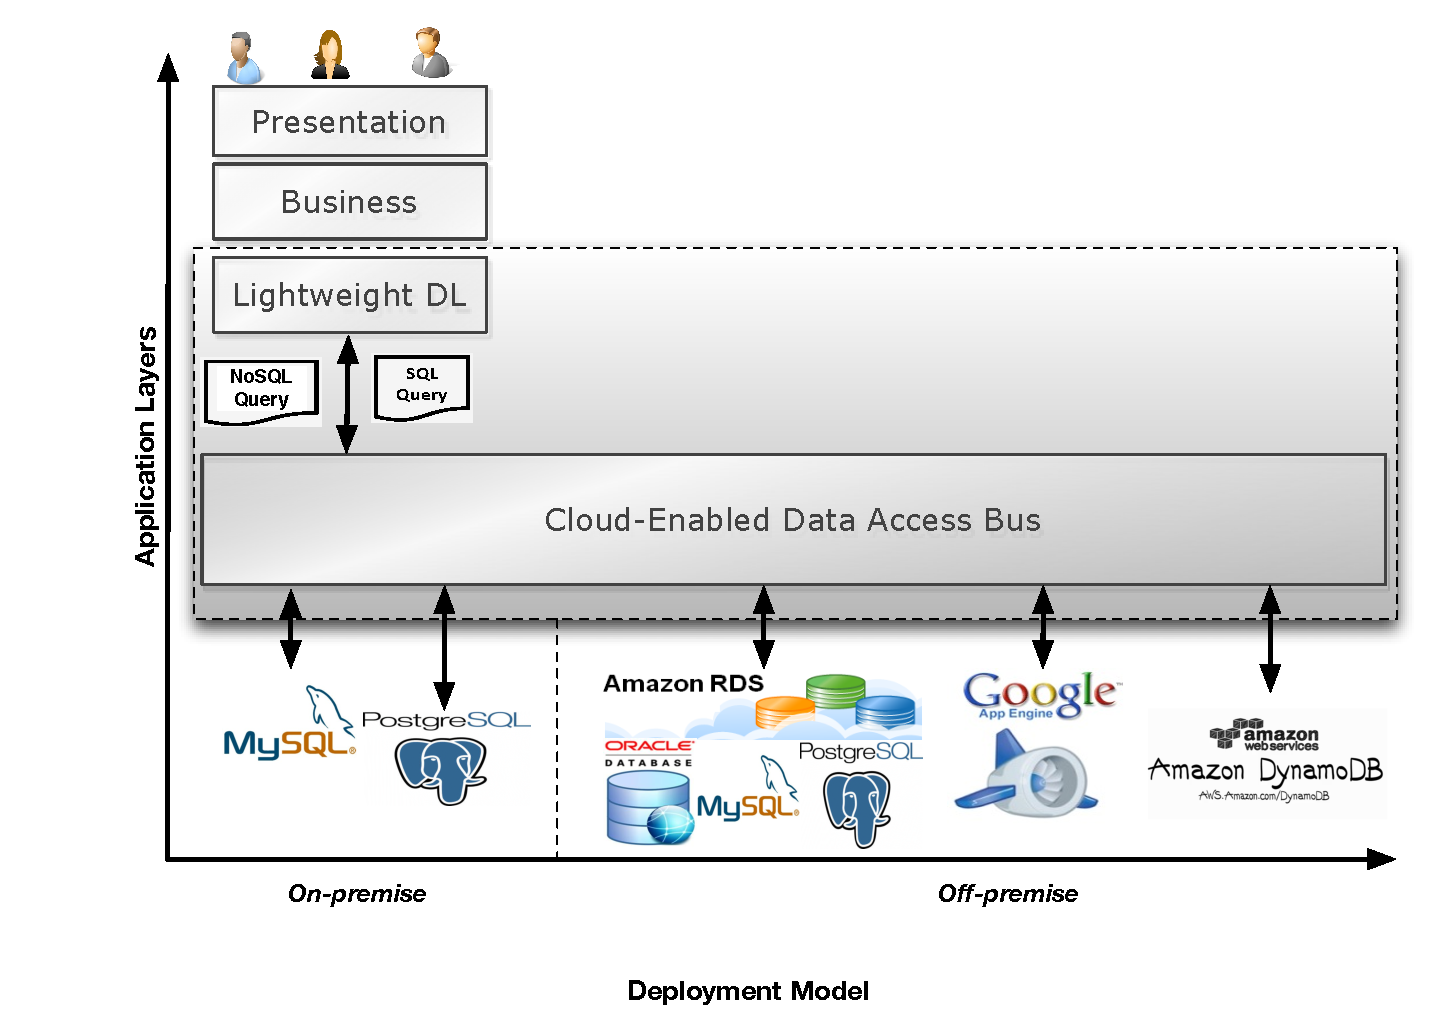
\includegraphics[width=0.925\textwidth, trim=0.0cm 0.0cm 0.0cm 0.0cm, clip]{./gfx/motivationScenario.pdf}
	\caption[Migration Scenario]{Migration Scenario to be filled }
	\label{fig:motivationscenario}
\end{figure}

As shown in Figure \ref{fig:motivationscenario}, the Cloud-Enabled Data Access bus provides access support between the hosted on-premise, and off-premise application's layers. Its main goal is to provide communication isolation between different applications and users, and maintain the transparency that the DL provided before the migration to the upper layers of the application's architecture. Support must be provided for two different databases types: MySQL and NoSQL databases, and between different providers. A tenant who migrates its data, e.g. to the Google SQL Datastore in Google App Engine, as shown in Figure \ref{fig:motivationscenario}, must be able to access his data with minimum adaptations of the components. Furthermore, storing or retrieving data whose storage is divided into multiple datasources requires a dynamic routing between backend data stores. Compatibility between different SQL and NoSQL databases must be also ensured. However, query and data transformation between different data sources types is out of the scope of this diploma thesis.  


\FloatBarrier
\section{Definitions and Conventions}
\label{sec:definitions}

In the following section we list the definitions and the abbreviations used in this diploma thesis for understanding the description of the work.

\subsection*{Definitions}

\subsection*{List of Abbreviations}

The following list contains abbreviations which are used in this document. 

\begin{acronym}[ApacheODEX]
\acro{ACID}{Atomicity, Consistency, Isolation, Durability}
              \acro{API}{Application Programming Interface}
	\acro{ASP}{Application Service Provider}
	\acro{Axis2}{Apache eXtensible Interaction System v. 2}
	\acro{BC}{Binding Component}
	\acro{BLOB}{Binary Large Object}
		\acro{BPEL}{Business Process Execution Language 2.0}
	\acro{C-CAST CMF}{Project Context Casting (C-CAST) Context-Management Framework}
		\acro{CLI}{Command-line Interface}
	\acro{CLOB}{Character Large Object}
	    \acro{CORBA}{Common Object Request Broker Architecture}
	         \acro{DBaaS}{Database-as-a-Service}
	           \acro{DBMS}{Database Management System}
	             \acro{DBS}{Database System}
	                  \acro{DCOM}{Distributed Component Object Model}
	                      \acro{DCE}{Distributed Computing Environment}
	\acro{EAI}{Enterprise Application Integration}
	\acro{EAR}{Enterprise Archive}
	\acro{EJB}{Enteprise JavaBeans}
	             \acro{EIP}{Enterprise Integration Patterns}
	\acro{ESB}{Enterprise Service Bus}
	        \acro{GAE}{Google App Engine}
	            \acro{HTTP}{Hypertext Transfer Protocol}
	\acro{IaaS}{Infrastructure-as-a-Service}
	\acro{IDE}{Integrated Development Environment}
	\acro{JAR}{Java Archive}
	\acro{Java EE 5}{Java Platform, Enterprise Edition v. 5}
	      \acro{J2EE}{Java 2 Platform, Enterprise Edition}
    \acro{JAX-WS}{Java API for XML-Based Web Services}
    \acro{JAXB}{Java Architecture for XML Binding}
	\acro{JBI}{Java Business Integration}
	\acro{JBIMulti2}{JBI Multi-tenancy Multi-container Support}
	\acro{JDBC}{Java Database Connectivity}
	\acro{JDK}{Java Development Kit}
	\acro{JMS}{Java Message Service}
	\acro{JMX}{Java Management Extensions}
	         \acro{JNDI}{Java Naming and Directory Interface} 
	\acro{JOnAS}{Java Open Application Server}
	\acro{JPA}{Java Persistence API}
	             \acro{JSON}{JavaScript Object Notation}
	\acro{JSF}{JavaServer Faces}
	\acro{JVM}{Java Virtual Machine}
	        \acro{LRU}{Least Recently Used} 
	\acro{MBean}{Managed Bean}
		\acro{MDBS}{Multidatabase System}
		       \acro{MEP}{Message Exchange Patterns}
		             \acro{MOM}{Message-Oriented Middleware}
	\acro{NIST}{National Institute of Standards and Technology}
	       \acro{NM}{Normalized Message}
	        \acro{NMF}{Normalized Message Format}
	\acro{NMR}{Normalized Message Router}
	               \acro{NoSQL}{Not only Structured Query Language}
	\acrodep{OSGi}{Open Services Gateway initiative}
	             \acro{ORDBMS}{Object-relational Database Management System}
	\acro{PaaS}{Platform-as-a-Service}
	\acro{POJO}{Plain Old Java Object}
	        \acro{POM}{Project Object Model}
	\acro{QoS}{Quality of Service}
	             \acro{RDBMS}{Relational Database Management System}
	                    \acro{SA}{Service Assembly}
	\acro{SaaS}{Software-as-a-Service}
    \acro{SE}{Service Engine}
            \acro{SMPP}{Short Message Peer-to-Peer}
            \acro{SNMP}{Simple Network Management Protocols}
	\acro{SOA}{Service-Oriented Architecture}
	\acrodep{SOAP}{Simple Object Access Protocol}
	              \acro{SQL}{Structured Query Language}
	              	          \acro{STaaS}{Storage-as-a-Service}
		                 \acro{SU}{Service Unit}
		\acro{TCP}{Transmission Control Protocol}
		       \acro{URI}{Uniform Resource Identifier}
    \acro{UUID}{Universally Unique Identifier}
    \acro{W3C}{World Wide Web Consortium}
            \acro{WAR}{Web Application Archive} 
    \acro{WS*}{Web Services (Specifications)}\acused{WS*}
    \acro{WSDL}{Web Services Description Language}
    \acro{WSS4J}{Apache Web Services Security for Java}
    \acro{XML}{eXtensible Markup Language}
    \acro{XSD}{XML Schema Definition}
    \acro{XSLT}{Extensible Stylesheet Language Transformation}
             

            

\end{acronym}
\section{Outline}
\label{sec:outline}

The remainder of this document is structured as follows:

\begin{itemize}
\item \textbf{Fundamentals, Chapter \ref{chap:fundamentals}:} provides the necessary background on the different concepts, technologies, and prototypes used in this diploma thesis.
\item \textbf{Related Works, Chapter \ref{chap:relatedworks}:} discusses relevant State of the Art and positions our work towards it.  
\item \textbf{Concept and Specification, Chapter \ref{chap:spec}:} functional and non-functional requirements are discussed in this section.
\item \textbf{Design, Chapter \ref{chap:design}:} gives a detailed overview of the differerent component's architecture, and the needed extensions to the already existing ones.
\item \textbf{Implementation, Chapter \ref{chap:implementation}:} the implemented components, as well as the necessary extensions or changes are detailed in this section from the point of view of coding and configuration. 
\item \textbf{Validation and Evaluation, Chapter \ref{chap:validationevaluation}:} in this chapter we test the final prototype based on the scenario described in this document. 
\item \textbf{Outcome and Future Work, Chapter \ref{chap:outcome}:} we provide a conclusion of the developed work and investigate some ideas in which this diploma thesis can be extended.
\end{itemize}